\subsection{飞行时间探测器}
\label{chap:TOF}
如上小节中所讨论,在动量相对较高的区间我们需要额外的信息来帮助进行粒子鉴别。飞行时间探测器(Time of Flight, ToF)被设计用来测量粒子的飞行速度从而进行粒子鉴别。这就对TOF的性能提出了如下要求:
\begin{itemize}
    \item 时间分辨率小于100ps, 对于停止时间(Stop time)的测量,时间分辨率应小于80ps。
    \item 每个通道的响应时间快,从而可以在在高粒子多重数的环境下工作
    \item 可以在STAR的磁场环境(0.5T)下稳定工作
    \item 成本相对较低,可以覆盖较大的范围从而与TPC中的径迹进行配对,空间接收度应与TPC类似。
\end{itemize}

基于这这些需求,多气隙电阻板室(Multi-gap Resistive Plate Chamber, MRPC)被用来作为TOF的终止时间测量探测器,起始时间由顶点位置探测器(Vertex Position Detector, VPD)给出。多气隙电阻板室首先被应用在ALICE实验上的时间飞行探测器当中,有着很高的时间分辨率且可以在高粒子多重数、强磁场的环境下工作。图 \ref{fig:MRPC} 为STAR中多气隙电阻板室的结构示意图。
\begin{figure}[htb]
    \begin{center}
    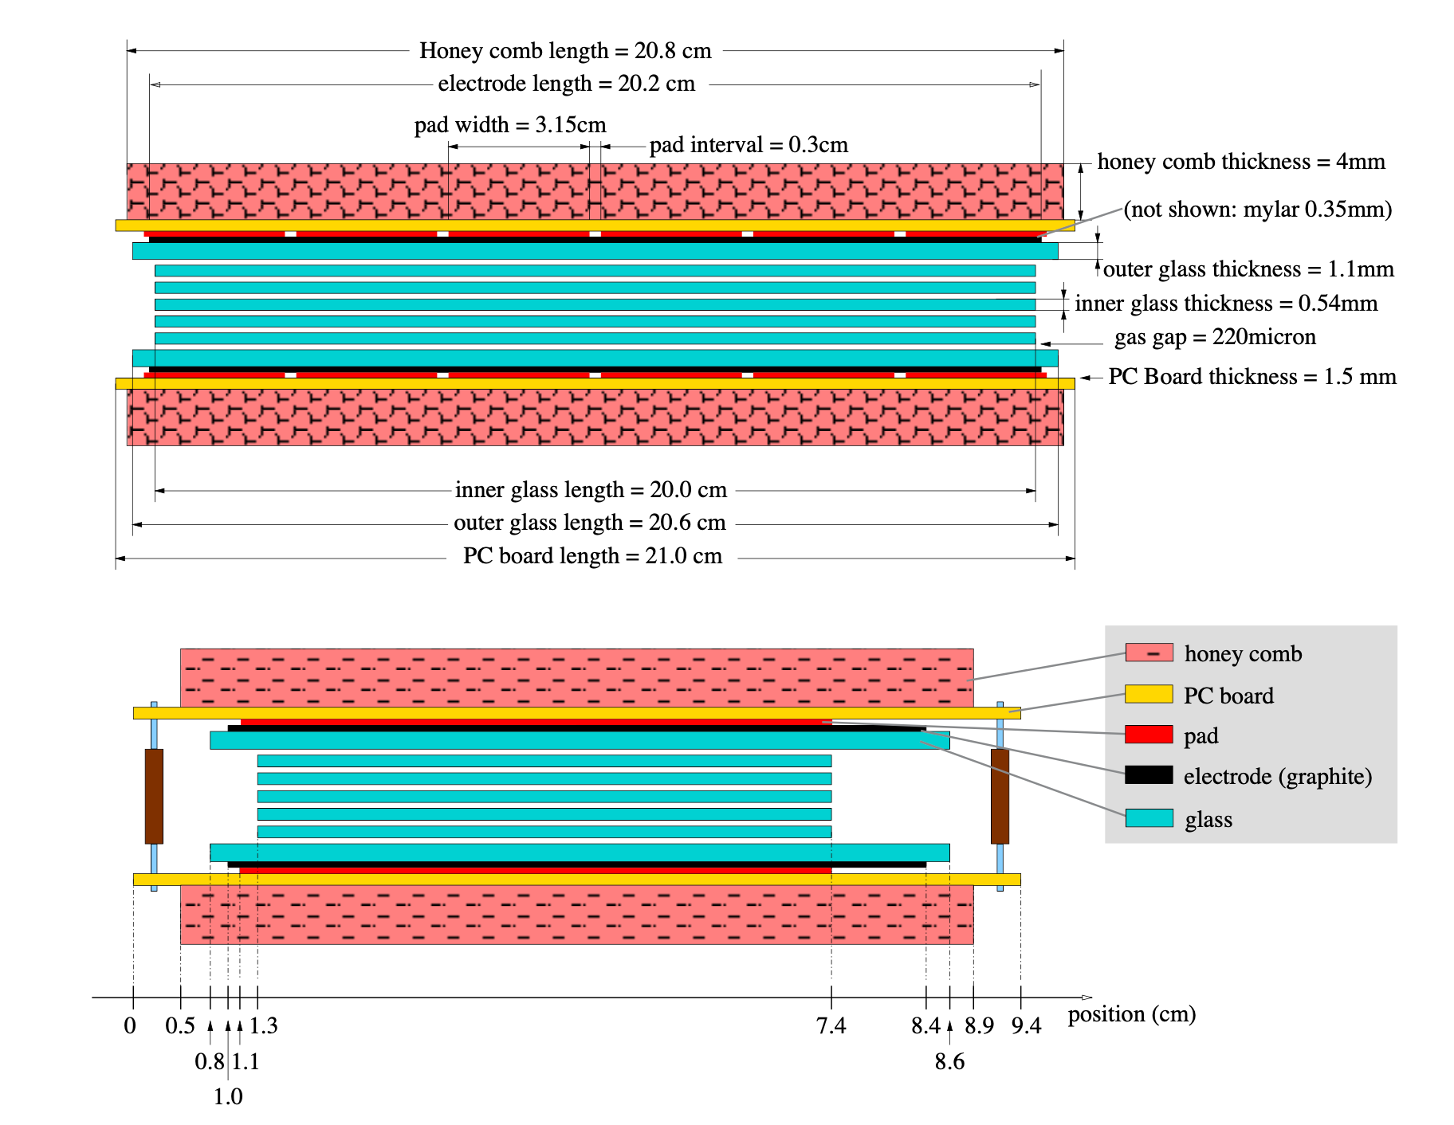
\includegraphics[width=0.7\textwidth,clip]{figures/Chapter2/MRPC.png}
    \end{center}
    \caption[MRPC结构示意图]{STAR上MRPC的测试图,上图为沿长边方向,下图为沿短边方向}
    \label{fig:MRPC}
\end{figure}
如图所示,在两个电极之间插入了5块阻性玻璃板,电极之间加有高压,可以在阻性板和阻性板之间的气隙之间产生高压。当带电粒子穿过整个室的时候可以在每个气隙处发生独立的雪崩过程。对于整个室而言,读出端所得到的感应信号相当于多个间隙内雪崩的“瞬时”叠加,因此可以获得一个相对较大的信号。多气隙电阻板室相对于传统的的阻性板室(Resistive Plate Chamber, RPC)计数率可以得到很大的提高。每个多气隙电阻板室具有6个 6.1 $\times$ 3.4cm 的读出pad,这使得飞行时间探测器的读出有着相对较好的读出粒度,使飞行时间探测器上的击中可以与时间投影室中的径迹进行配对。飞行时间探测器安装在时间投影室桶部外部,其接收度和时间投影室类似,也有着全方位角($ 0 < \phi < 2\pi$)和中心快度区间($ |\eta| < 0.9 $)的接收度。

结合多气隙电阻板室测得的终止时间和顶点位置探测器测得的起始时间可以得到径迹的飞行时间,再利用时间投影室测量得到的径迹长度信息可以计算得到粒子的飞行速度用以进行粒子鉴别,图 \ref{fig:TOFPerformance} 展示了TOF测量的 $1/\beta$ 随动量变化的分布以及添加 $1/\beta$ 判选条件后的电离能损分布。可以看到,在额外添加$|1-1/\beta| < 0.03$的判选条件时,电子的电离能损可以很好的与其他粒子区分开来。整个STAR探测器的粒子鉴别能力在添加径迹的速度信息后得到了很好的提升。

\begin{figure}[htb]
    \centering
    \begin{subfigure}[b]{0.47\textwidth}
        \centering
        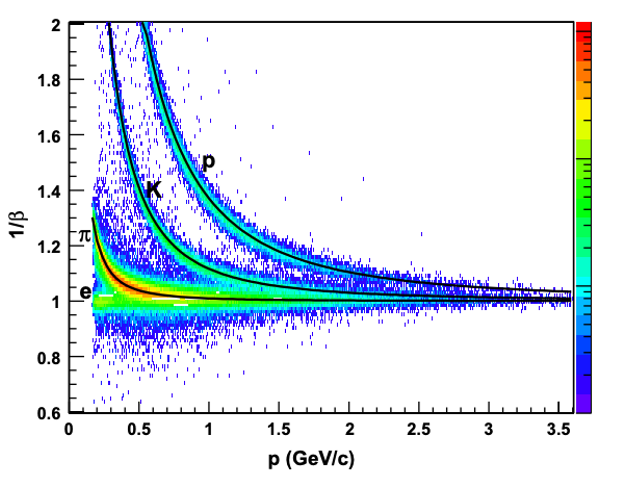
\includegraphics[width=0.9\textwidth,clip]{figures/Chapter2/BetaDistribution.png}
        \caption{}
        \label{fig:BetaDis}
    \end{subfigure}
    \hfill
    \begin{subfigure}[b]{0.47\textwidth}
        \centering
        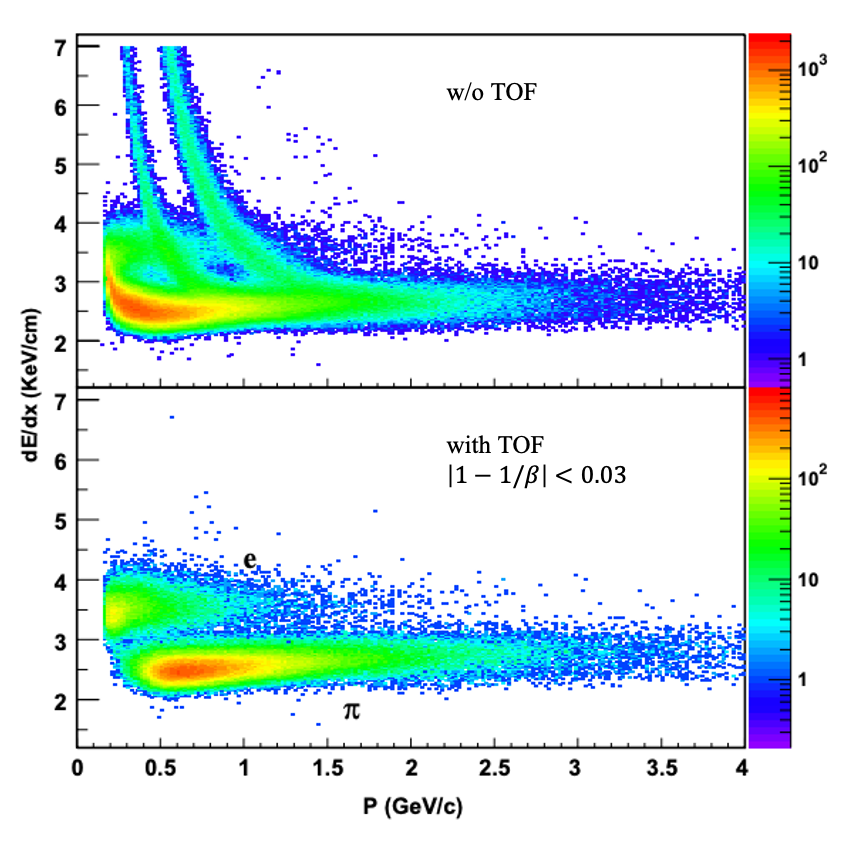
\includegraphics[width=0.9\textwidth,clip]{figures/Chapter2/dEdxwithTOF.png}
        \caption{}
        \label{fig:dEdxwithTOF}
    \end{subfigure}
       \caption[飞行时间探测器粒子鉴别表现]{图(a)粒子的$1/\beta$分布随着动量变化的示意图。图(b)为电离能损(dE/dx)随着动量变化的分布。上半部分为仅用时间投影室测量,不添加额外的关于$\beta$的判选条件的电离能损分布。下半部分为在上半部分基础上额外添加 $|1-1/\beta| < 0.03$的判选条件时的电离能损分布}
       \label{fig:TOFPerformance}
\end{figure}
  